\subsection{Cel opracowania}

Dokument ma na celu efektywnie (tj. jak najmniejszym nakładem czasu wymaganym do uzyskania satysfakcjonujących wyników) zademonstrować możliwości środowiska \LaTeX\ skutkującym umiejętnością tworzenia dobrej jakości dokumentów, z którymi Studenci spotykają się na co dzień:

\begin{itemize}
	\item \textbf{raportów},
	\item \textbf{sprawozdań},
	\item instrukcji,
	\item prac dyplomowych,
	\item skryptów. 
\end{itemize}

Bez konieczności szczegółowego zagłębiania się w tajniki składni \LaTeX\ możliwe jest tworzenie własnych dokumentów z wykorzystaniem niniejszej bazy przez zastosowanie analogii. W opracowaniu zwrócono uwagę na:

\begin{itemize}
	\item proces instalacji wymaganych do pracy elementów,
	\item początkową konfigurację środowiska,
	\item główne elementy składowe opracowania techniczno-naukowego (akapity, poziomy tekstu tj. rozdział, sekcja, podsekcja, listy, rysunki, formuły matematyczne, tabele, wyciągi z kodów, bibliografia) wraz z przykładami stosowania najbardziej oczywistych/ najczęściej stosowanych konfiguracjach.
\end{itemize}

Powyższe pozwala na niemal natychmiastowe rozpoczęcie korzystania z możliwości składania tekstu w środowisku \LaTeX. 

Autor zakłada, że Czytelnik szybko przekona się do korzyści jakie płyną ze stosowania tego typu narzędzi coraz rzadziej sięgając po systemy edytorów typu WYSIWYG.

\subsection{Narzędzia i źródła}

Opisywane w dokumencie środowisko do zautomatyzowanego składu tekstu \LaTeX\ łączy dwa elementy:

\begin{itemize}
	\item zestaw plików wykonawczych/binarnych wraz z pakietami oraz niezbędnymi zależnościami, dla MS Windows będzie to MiKTeX \cite{noauthor_home_nodate}, \cite{noauthor_getting_nodate} (\url{https://miktex.org/download}),
	\item edytora składni \LaTeX\ , w opisywanym przykładzie użyto TeXnicCenter \cite{noauthor_texniccenter_nodate}, \cite{noauthor_texniccenter_nodate-1} (\url{https://www.texniccenter.org/download/}).
\end{itemize}

Środowisko MiKTeX można pobrać w formie pliku instalacyjnego tzw. \textit{Basic Installer} (240.1 MB) lub zainstalować pełen pakiet za pośrednictwem \textit{Net Installer} (23.77 MB). Sugeruje się instalację podstawowej wersji (\textit{Basic Installer}), jako że w przypadku napotkania w składni na brakujący pakiet środowisko podejmie próbę jego doinstalowania. 

Zarządzanie zainstalowanymi pakietami MiKTeX możliwe jest (w nowszych wersjach) za pośrednictwem aplikacji \textit{MiKTeX Console} (sugeruje się uruchamiać w trybie administratora). Stanowi ona integralną część środowiska MiKTeX -- także w wersji podstawowej.
 
\subsection{Instalacja}

Aby instalacja przebiegała bez większych problemów, należy w pierwszej kolejności zainstalować pakiet MiKTeX, a następnie TeXnicCenter (dzięki temu automatycznie zostanie zlokalizowany folder z plikami wykonawczymi). W przypadku, gdy edytor nie rozpozna poprawnie położenia tych plików, należy wskazać je samodzielnie (w katalogu instalacji MiKTeX np.: \url{U:\LaTeX\miktex\bin\x64\}). 

\subsection{Ustawienia początkowe}

Podany przykład dokumentu celem poprawnej kompilacji \textcolor[rgb]{1,0,0}{\textbf{WYMAGA}} modyfikacji parametrów wywołania kompilatora \LaTeX\  tj. pole \textit{Command line to pass to the compiler} jak pokazano na rysunku \ref{fig:build01}.
Okno dostępne jest z poziomu menu \textit{Build --> Define output profiles}.

\begin{lstlisting}[language=TeX, frame=single, caption = {Zawartość pola \textit{Command line arguments to pass to the compiler}}, label = {}]
-shell-escape -synctex=-1 -max-print-line=120 -interaction=nonstopmode "%wm" 
\end{lstlisting}


 \begin{figure}[ht]
  \centering
  \resizebox{120mm}{!}{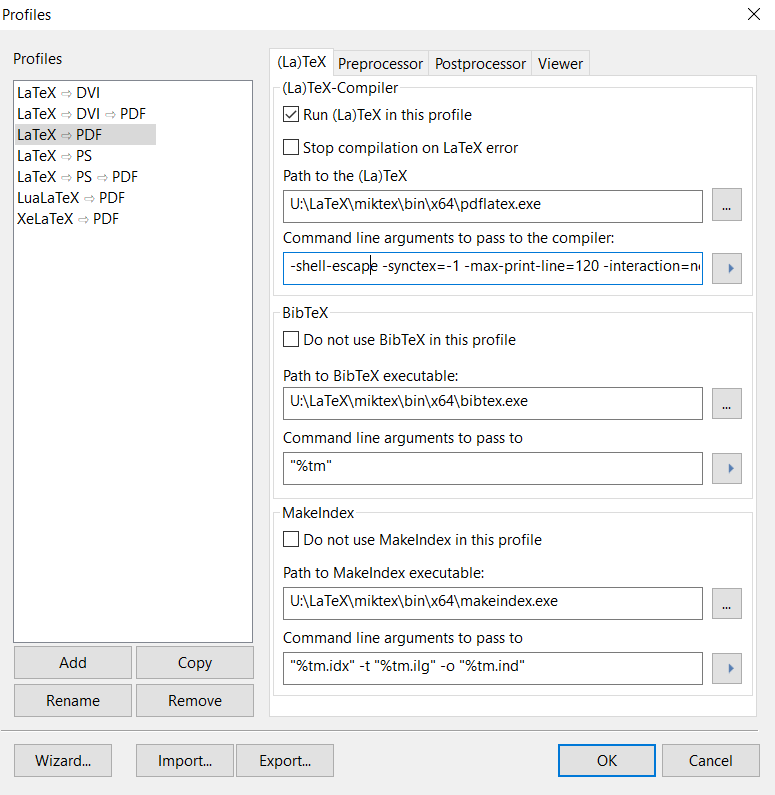
\includegraphics{img/conf.png}}
  \caption{Okno konfiguracji budowania wg profilu LaTeX --> PDF (źródło: opracowanie własne)}
  \label{fig:build01}
\end{figure}

Należy zwrócić uwagę, aby pliki źródłowe \LaTeX\ zapisywane były w odpowiednim formacie zdefiniowanym w ustawieniach interpretera (w opisywanym przypadku jest to UTF-8). Przy zapisie pliku w MS Windows menu \textit{File->Save As} należy zwrócić uwagę na pola \textit{File format} oraz \textit{Encoding} zgodnie z rysunkiem \ref{fig:save01}.


\begin{figure}[ht]
  \centering
  \resizebox{160mm}{!}{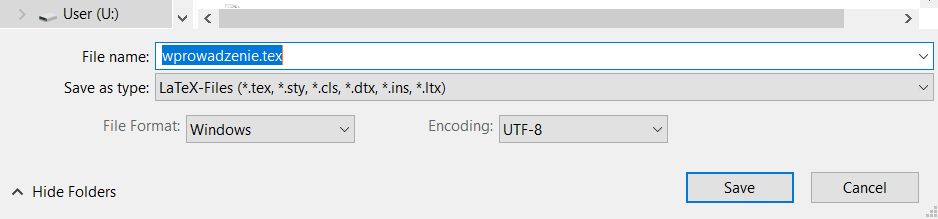
\includegraphics{img/wprowadzenie.png}}
  \caption{Opcje zapisu pliku źródłowego TeX (źródło: opracowanie własne)}
  \label{fig:save01}
\end{figure}

